\documentclass[12pt]{article}
\usepackage[margin=1in]{geometry}
\usepackage{amsmath,amssymb,mathtools}
\usepackage{booktabs}
\usepackage{enumitem}
\usepackage{bm}
\usepackage{hyperref}
\usepackage{fancyhdr}
\usepackage{draftwatermark}
\usepackage{xcolor}
\usepackage{pgfplots}
\usepackage{titlesec}
\pgfplotsset{compat=newest}

%------------- TITLE AND METADATA -------------
\newcommand{\CourseCode}{HE2001 }
\newcommand{\CourseName}{Microeconomics II}
\newcommand{\DocType}{Tutorial 10}

\title{
\CourseCode \CourseName \\[0.3em]
\large \DocType
}
\author{
  Academic Year 2025/2026, Semester 2 \\[0.25em]
  \textit{Quantitative Research Society @NTU}
}
\date{\today}

%------------- HEADER & FOOTER (for page 2 onward) -------------
\fancypagestyle{main}{
  \fancyhf{}
  \fancyhead[L]{\CourseCode \CourseName \ --\ \DocType}
  \fancyhead[R]{\href{https://qrsntu.org}{QRS@NTU}}
  \fancyfoot[C]{\thepage}
  \renewcommand{\headrulewidth}{0.4pt}
  \renewcommand{\footrulewidth}{0pt}
}

%------------- SIMPLE FOOTER (page 1 only) -------------
\fancypagestyle{plainfirst}{
  \fancyhf{}
  \renewcommand{\headrulewidth}{0pt}
  \renewcommand{\footrulewidth}{0pt}
  \fancyfoot[C]{\scriptsize\textcolor{gray}{\textit{For academic reference only. This document is provided for educational purposes and does not constitute an official question paper, answer key, or any formally authorised academic material. Its content is not guaranteed to be complete or accurate.}}}
}

%------------- WATERMARK -------------
\SetWatermarkText{Unofficial — QRS@NTU — qrsntu.org}
\SetWatermarkScale{1}
\SetWatermarkLightness{0.99}

%------------- SHORTCUTS -------------
\newcommand{\R}{\mathbb{R}}
\newcommand{\Rp}{\mathbb{R}_+}
\newcommand{\E}{\mathbb{E}}
\newcommand{\Var}{\mathrm{Var}}
\newcommand{\dotp}{\cdot}

%------------- STYLE -------------
\setlist[enumerate]{itemsep=0.32em, topsep=0.32em}
\setlist[itemize]{itemsep=0.22em, topsep=0.22em}

\titleformat{\subsubsection}[block]
{\normalfont\large\bfseries}
{}
{0pt}
{}

\titleformat{\paragraph}[block]
{\normalfont\normalsize\bfseries}
{}
{0pt}
{}

\titlespacing*{\paragraph}
{0pt}
{1.2ex}
{0.6ex}

\setcounter{secnumdepth}{0}
\setcounter{tocdepth}{4}

\begin{document}

\maketitle
\thispagestyle{plainfirst}
\pagestyle{main}
\bigskip

%====================================================
% OVERVIEW
%====================================================
\begin{center}
  \rule{0.8\textwidth}{0.4pt}\\[4pt]
  \textbf{Overview}\\[2pt]
  \rule{0.8\textwidth}{0.4pt}
\end{center}

\noindent
This tutorial covers:
\begin{itemize}[leftmargin=*]
  \item plurality voting and Borda count as social decision mechanisms;
  \item completeness, transitivity, the Pareto condition, and independence of irrelevant alternatives;
  \item strategic incentives under rank-based voting rules;
  \item utility possibility frontiers and their slopes;
  \item utilitarian, weighted-utilitarian, Nietzschean, Rawlsian, and Cobb--Douglas social welfare functions;
  \item graphical and analytical characterisation of socially optimal utility allocations.
\end{itemize}

\bigskip

\newpage
\tableofcontents

\newpage
%====================================================
% QUESTION 1
%====================================================
\section{Question 1: Plurality Voting}

\noindent
Consider Plurality Voting as discussed in the lecture.\footnote{Suppose that there are $n$ alternatives. Given the $n$ alternatives, pick the alternative that is the top choice of the largest number of individuals and place it at the top of the social preference ordering. Ties are broken randomly. Then, remove that alternative from every individual's preference ordering, keeping the same order for the $n-1$ remaining alternatives. (For example, if $a \succ_i b \succ_i c$, and we are removing alternative $b$ which was the top, then it becomes $a \succ_i c$.) Repeat the above process on the remaining alternatives until only one remains which is the bottom of the social preference ordering.} Suppose that there are a finite number of alternatives and that everyone has rational and strict preferences.

\subsection{Problem}
\begin{enumerate}[label=(\alph*)]
    \item Will the plurality voting social decision mechanism always result in a complete and transitive social preference ordering? Explain.
    \item Does plurality voting satisfy the pareto condition? Explain.
    \item Consider the case of 3 alternatives and a society with 9 individuals with the following preference list:
    \begin{itemize}[leftmargin=2em]
        \item 4 individuals have $A \succ_i B \succ_i C$
        \item 3 individuals have $C \succ_i B \succ_i A$
        \item 2 individuals have $B \succ_i A \succ_i C$
    \end{itemize}
    What is the social ranking according to the plurality voting?
    \item Now, suppose we swap the middle 3 individuals' preferences over $B$ and $C$ such that the preference list becomes:
    \begin{itemize}[leftmargin=2em]
        \item 4 individuals have $A \succ_i B \succ_i C$
        \item 3 individuals have $B \succ_i C \succ_i A$
        \item 2 individuals have $B \succ_i A \succ_i C$
    \end{itemize}
    What is the social ranking according to plurality voting?
    \item Does the plurality voting social decision mechanism satisfy the requirement of independence of irrelevant alternatives? Hint: use parts c) and d).
\end{enumerate}

\newpage
\subsection{Solution}

\subsubsection{Method 1: Recursive winner-elimination method}

\begin{enumerate}[label=(\alph*)]
    \item
    Yes. At each stage of the plurality procedure, one of the remaining alternatives is selected and placed next in the social ordering.

    There are only finitely many alternatives. Therefore the procedure cannot continue forever: after one alternative is chosen, the number of remaining alternatives falls by one, and after finitely many steps exactly one alternative remains.

    Hence the procedure always produces an ordered list of all alternatives, say
    \[
    x_1 \succ x_2 \succ \cdots \succ x_n.
    \]
    Because every pair of alternatives appears somewhere in this list, the social ordering is complete. Because the ranking is literally a single ordered list, it is also transitive: whenever
    \[
    x_i \succ x_j \quad\text{and}\quad x_j \succ x_k,
    \]
    we automatically have
    \[
    x_i \succ x_k.
    \]
    Therefore plurality voting always yields
    \[
    \boxed{\text{a complete and transitive social preference ordering.}}
    \]

    \item
    Yes. Suppose every individual strictly prefers some alternative $X$ to another alternative $Y$.

    Consider any round of the plurality procedure in which both $X$ and $Y$ are still present. Since every person ranks $X$ above $Y$, it is impossible for $Y$ to be anyone's top-ranked remaining option unless $X$ has already been removed earlier.

    But that earlier removal would mean that $X$ had already been placed socially above $Y$. Therefore there is no possible stage at which $Y$ can be placed above $X$ while $X$ remains below it.

    Hence plurality voting respects unanimous strict preferences:
    \[
    \boxed{\text{If everyone prefers }X\text{ to }Y,\text{ then society ranks }X\text{ above }Y.}
    \]
    So the Pareto condition is satisfied.

    \item
    In the first round, the first-place vote totals are:
    \[
    A:4,\qquad B:2,\qquad C:3.
    \]
    Hence $A$ has the largest number of first-place votes, so $A$ is placed first socially.

    Remove $A$ from every ranking. The remaining rankings become:
    \begin{itemize}[leftmargin=2em]
        \item 4 individuals: $B \succ_i C$
        \item 3 individuals: $C \succ_i B$
        \item 2 individuals: $B \succ_i C$
    \end{itemize}
    So the new first-place totals are:
    \[
    B:6,\qquad C:3.
    \]
    Hence $B$ is placed second and $C$ last.

    Therefore the plurality-voting social ranking is
    \[
    \boxed{A \succ B \succ C.}
    \]

    \item
    Now the first-round first-place vote totals are:
    \[
    A:4,\qquad B:5,\qquad C:0.
    \]
    Hence $B$ is placed first socially.

    Remove $B$ from every ranking. The remaining rankings become:
    \begin{itemize}[leftmargin=2em]
        \item 4 individuals: $A \succ_i C$
        \item 3 individuals: $C \succ_i A$
        \item 2 individuals: $A \succ_i C$
    \end{itemize}
    So the new first-place totals are:
    \[
    A:6,\qquad C:3.
    \]
    Hence $A$ is placed second and $C$ last.

    Therefore the social ranking is
    \[
    \boxed{B \succ A \succ C.}
    \]

    \item
    Independence of irrelevant alternatives requires that if every individual's ranking between $A$ and $B$ stays unchanged, then the social ranking between $A$ and $B$ should also stay unchanged.

    Compare parts (c) and (d). In both profiles:
    \begin{itemize}[leftmargin=*]
        \item the 4 individuals still rank $A$ above $B$;
        \item the 3 middle individuals still rank $B$ above $A$;
        \item the 2 remaining individuals still rank $B$ above $A$.
    \end{itemize}
    So nobody changed their relative ranking of $A$ and $B$.

    However, the social ranking between $A$ and $B$ changed:
    \[
    A \succ B \quad\text{in part (c),}
    \qquad
    B \succ A \quad\text{in part (d).}
    \]
    Hence plurality voting does not satisfy independence of irrelevant alternatives.

    Therefore
    \[
    \boxed{\text{Plurality voting violates IIA.}}
    \]
\end{enumerate}

\subsubsection{Method 2: Top-count tables and contradiction argument}

\begin{enumerate}[label=(\alph*)]
    \item
    The plurality rule sequentially assigns first place, then second place, and so on, until every alternative has been assigned a position. This necessarily generates one ranked list of all alternatives. Any such ranked list is complete and transitive. Hence
    \[
    \boxed{\text{plurality voting always gives a complete and transitive ordering.}}
    \]

    \item
    Suppose everybody ranks $X$ above $Y$. Then whenever both $X$ and $Y$ remain under consideration, $Y$ cannot receive more top rankings than $X$, because $Y$ is never above $X$ in any person's list. So $Y$ cannot be placed socially above $X$. Hence the Pareto condition holds:
    \[
    \boxed{X \succ Y \text{ socially whenever all individuals have } X \succ_i Y.}
    \]

    \item
    The plurality table for the original profile is
    \[
    \begin{array}{c|ccc}
    \text{Round 1} & A & B & C\\ \hline
    \text{Top votes} & 4 & 2 & 3
    \end{array}
    \]
    so $A$ is first.

    After removing $A$,
    \[
    \begin{array}{c|cc}
    \text{Round 2} & B & C\\ \hline
    \text{Top votes} & 6 & 3
    \end{array}
    \]
    so $B$ is second and $C$ third. Thus
    \[
    \boxed{A \succ B \succ C.}
    \]

    \item
    The plurality table for the modified profile is
    \[
    \begin{array}{c|ccc}
    \text{Round 1} & A & B & C\\ \hline
    \text{Top votes} & 4 & 5 & 0
    \end{array}
    \]
    so $B$ is first.

    After removing $B$,
    \[
    \begin{array}{c|cc}
    \text{Round 2} & A & C\\ \hline
    \text{Top votes} & 6 & 3
    \end{array}
    \]
    so $A$ is second and $C$ third. Thus
    \[
    \boxed{B \succ A \succ C.}
    \]

    \item
    In parts (c) and (d), all individuals keep the same relative ordering of $A$ and $B$, but the social ordering between $A$ and $B$ reverses. Therefore plurality voting depends on changes involving the third option $C$, which is exactly what IIA forbids. Hence
    \[
    \boxed{\text{plurality voting fails IIA.}}
    \]
\end{enumerate}

%====================================================
% QUESTION 2
%====================================================
\newpage
\section{Question 2: Borda Count}

\noindent
Consider the Borda Count as discussed in the lecture. Suppose that there are a finite number of alternatives and that everyone has rational and strict preferences.

\subsection{Problem}
\begin{enumerate}[label=(\alph*)]
    \item Will the Borda Count social decision mechanism always result in a complete and transitive social preference ordering? Explain.
    \item Does the Borda Count social decision mechanism defined in this way satisfy the pareto condition? Explain.
    \item Suppose that there are two voters and three candidates, $x$, $y$, and $z$. Suppose that Voter 1 ranks the candidates: $x$ first, $z$ second, and $y$ third. Suppose that Voter 2 ranks the candidates: $y$ first, $x$ second, and $z$ third. What is the Borda count for $x$, $y$ and $z$?
    \item Now suppose that it is discovered that candidate $z$ once lifted a beagle by the ears. Voter 1, who has rather large ears himself, is appalled and changes his ranking to $x$ first, $y$ second, $z$ third. Voter 2, who picks up his own children by the ears, is favorably impressed and changes his ranking to $y$ first, $z$ second, $x$ third. What is the Borda count for $x$, $y$ and $z$?
    \item Does the Borda Count social decision mechanism satisfy independence of irrelevant alternatives? Hint: use parts d) and e).
    \item Do you think that with Borda Voting, voters always have an incentive to truthfully report their full preference rankings? (Hint: provide an example where a voter changes his reported ranking and benefits from it)
\end{enumerate}

\newpage
\subsection{Solution}

\subsubsection{Method 1: Score-summation method}

\begin{enumerate}[label=(\alph*)]
    \item
    Yes. Under the Borda Count, every alternative receives a total score obtained by summing the points assigned by all voters.

    Because the number of voters and alternatives is finite, every alternative has a well-defined total score. Comparing total scores yields a social ordering: the alternative with the smaller total score is socially preferred, and equal total scores imply social indifference under this version of the rule.

    Since ordinary numerical comparison is complete and transitive, the induced social ordering is also complete and transitive. Therefore
    \[
    \boxed{\text{the Borda Count always produces a complete and transitive social preference ordering.}}
    \]

    \item
    Yes. Suppose every voter ranks $x$ above $y$.

    Under the Borda Count, a higher-ranked alternative receives a strictly better score from each individual than a lower-ranked alternative. Therefore each voter assigns fewer points to $x$ than to $y$. Summing across all voters preserves this strict inequality, so the total score of $x$ is smaller than the total score of $y$.

    Since lower total score is socially better, society ranks $x$ above $y$. Hence the Borda Count satisfies the Pareto condition:
    \[
    \boxed{\text{If every voter ranks }x\text{ above }y,\text{ then society ranks }x\text{ above }y.}
    \]

    \item
    With three candidates, assign 1 point to first place, 2 points to second place, and 3 points to third place.

    Voter 1 has
    \[
    x \succ z \succ y,
    \]
    so contributes
    \[
    x:1,\qquad z:2,\qquad y:3.
    \]
    Voter 2 has
    \[
    y \succ x \succ z,
    \]
    so contributes
    \[
    y:1,\qquad x:2,\qquad z:3.
    \]
    Summing these scores:
    \[
    x:1+2=3,
    \qquad
    y:3+1=4,
    \qquad
    z:2+3=5.
    \]
    Therefore the Borda counts are
    \[
    \boxed{x:3,\qquad y:4,\qquad z:5.}
    \]
    Since lower score is better, the social ranking is
    \[
    \boxed{x \succ y \succ z.}
    \]

    \item
    Under the revised rankings,
    \[
    \text{Voter 1: } x \succ y \succ z,
    \qquad
    \text{Voter 2: } y \succ z \succ x.
    \]
    So Voter 1 contributes
    \[
    x:1,\qquad y:2,\qquad z:3,
    \]
    and Voter 2 contributes
    \[
    y:1,\qquad z:2,\qquad x:3.
    \]
    Summing:
    \[
    x:1+3=4,
    \qquad
    y:2+1=3,
    \qquad
    z:3+2=5.
    \]
    Therefore the Borda counts are
    \[
    \boxed{x:4,\qquad y:3,\qquad z:5.}
    \]
    Hence the social ranking is
    \[
    \boxed{y \succ x \succ z.}
    \]

    \item
    No. Compare parts (c) and (d). Nobody changed their mind about the relative ordering of $x$ and $y$:
    \begin{itemize}[leftmargin=*]
        \item Voter 1 ranks $x$ above $y$ in both cases.
        \item Voter 2 ranks $y$ above $x$ in both cases.
    \end{itemize}
    So each voter's preferences between $x$ and $y$ are unchanged.

    However, the social ranking between $x$ and $y$ changes:
    \[
    x \succ y \quad\text{in part (c),}
    \qquad
    y \succ x \quad\text{in part (d).}
    \]
    The change arose only because the position of the third candidate $z$ changed. Therefore Borda Count violates independence of irrelevant alternatives:
    \[
    \boxed{\text{Borda Count does not satisfy IIA.}}
    \]

    \item
    No. Voters do not always have an incentive to report truthfully.

    Consider the following true preferences of three voters over four alternatives $X,Y,Z,W$:
    \[
    \begin{array}{c|ccc}
    \text{Rank} & \text{Bill} & \text{Bertha} & \text{Bob} \\ \hline
    1 & X & Y & Z \\
    2 & Y & Z & X \\
    3 & Z & X & Y \\
    4 & W & W & W
    \end{array}
    \]
    With four alternatives, assign 1 point to first place, 2 to second, 3 to third, and 4 to fourth. Under truthful reporting the totals are
    \[
    X:1+3+2=6,
    \qquad
    Y:2+1+3=6,
    \qquad
    Z:3+2+1=6,
    \qquad
    W:4+4+4=12.
    \]
    So $X,Y,Z$ tie for the best score. If ties are broken randomly, Bertha faces an equal-chance outcome among $X,Y,Z$.

    Now suppose Bertha strategically reports
    \[
    Y \succ W \succ Z \succ X
    \]
    instead of her true ranking
    \[
    Y \succ Z \succ X \succ W.
    \]
    Then the reported profile becomes
    \[
    \begin{array}{c|ccc}
    \text{Rank} & \text{Bill} & \text{Bertha} & \text{Bob} \\ \hline
    1 & X & Y & Z \\
    2 & Y & W & X \\
    3 & Z & Z & Y \\
    4 & W & X & W
    \end{array}
    \]
    and the totals become
    \[
    X:1+4+2=7,
    \qquad
    Y:2+1+3=6,
    \qquad
    Z:3+3+1=7,
    \qquad
    W:4+2+4=10.
    \]
    So $Y$ becomes the unique social winner.

    Since Bertha's true ranking has $Y$ as her top choice, she strictly prefers this manipulated outcome to the truthful tie among $X,Y,Z$. Hence she benefits from misreporting.

    Therefore
    \[
    \boxed{\text{Borda voting is not strategy-proof; voters may gain from lying.}}
    \]
\end{enumerate}

\subsubsection{Method 2: Rank-order proof and explicit manipulation example}

\begin{enumerate}[label=(\alph*)]
    \item
    The Borda rule converts each preference profile into a vector of total scores. Ordering alternatives by their total scores gives a social ranking. Because real numbers are completely and transitively ordered, the resulting social preference relation is complete and transitive. Thus
    \[
    \boxed{\text{the Borda Count always yields a complete and transitive ordering.}}
    \]

    \item
    If every voter ranks $x$ above $y$, then $x$ receives a better rank than $y$ from every voter, hence fewer Borda points from every voter, and therefore fewer total points overall. So society ranks $x$ above $y$. Hence
    \[
    \boxed{\text{the Borda Count satisfies the Pareto condition.}}
    \]

    \item
    Under the original profile, the score table is
    \[
    \begin{array}{c|ccc}
    & x & y & z \\ \hline
    \text{Voter 1} & 1 & 3 & 2 \\
    \text{Voter 2} & 2 & 1 & 3 \\ \hline
    \text{Total} & 3 & 4 & 5
    \end{array}
    \]
    so
    \[
    \boxed{x \succ y \succ z.}
    \]

    \item
    Under the revised profile, the score table is
    \[
    \begin{array}{c|ccc}
    & x & y & z \\ \hline
    \text{Voter 1} & 1 & 2 & 3 \\
    \text{Voter 2} & 3 & 1 & 2 \\ \hline
    \text{Total} & 4 & 3 & 5
    \end{array}
    \]
    so
    \[
    \boxed{y \succ x \succ z.}
    \]

    \item
    The relative individual ranking between $x$ and $y$ is unchanged between parts (c) and (d), yet the social ranking flips from $x \succ y$ to $y \succ x$. Therefore the rule depends on changes in the position of $z$, which means
    \[
    \boxed{\text{Borda Count fails IIA.}}
    \]

    \item
    The strategic example in Method 1 proves that truthful revelation need not be optimal. The key mechanism is that under Borda Count, changing the reported ranking of lower alternatives changes their scores and can alter the winner, even when the voter's favourite remains at the top. Thus
    \[
    \boxed{\text{voters may benefit from misreporting under Borda voting.}}
    \]
\end{enumerate}

%====================================================
% QUESTION 3
%====================================================
\newpage
\section{Question 3: Norton, Ralph, and the Utility Possibility Frontier}

\noindent
Norton and Ralph have a utility possibility frontier that is given by the following equation,
\[
U_R + U_N^2 = 100
\]
(where $R$ and $N$ signify Ralph and Norton respectively).

\subsection{Problem}
\begin{enumerate}[label=(\alph*)]
    \item If we set Norton's utility to zero, what is the highest possible utility Ralph can achieve? If we set Ralph's utility to zero, what is the best Norton can do?
    \item Plot the utility possibility frontier on a graph.
    \item Derive an equation for the slope of the above utility possibility curve.
    \item Suppose that a social planner who is deciding on the allocation of Ralph and Norton has a utilitarian social welfare function. What is the utility of Ralph and Norton in the social planner's ideal allocation?
    \item Both Ralph and Norton believe that the ideal allocation is given by maximizing an appropriate social welfare function. Ralph thinks that $U_R=75,U_N=5$ is the best distribution of welfare, and presents the maximization solution to a weighted-sum-of-the-utilities social welfare function that confirms this observation. What was Ralph's social welfare function?

    (Hint: What is the slope of Ralph's social welfare function?)
    \item Norton, on the other hand, believes that $U_R=19,U_N=9$ is the best distribution. What was Norton's social welfare function?
\end{enumerate}

\newpage
\subsection{Solution}

\subsubsection{Method 1: Frontier substitution and tangency conditions}

\begin{enumerate}[label=(\alph*)]
    \item
    The utility possibility frontier is
    \[
    U_R + U_N^2 = 100.
    \]

    If $U_N=0$, then
    \[
    U_R = 100-0^2=100.
    \]
    Hence the highest utility Ralph can achieve is
    \[
    \boxed{U_R=100.}
    \]

    If $U_R=0$, then
    \[
    U_N^2=100.
    \]
    Taking the nonnegative value relevant for utility,
    \[
    U_N=10.
    \]
    Hence the best Norton can do is
    \[
    \boxed{U_N=10.}
    \]

    \item
    Rewrite the frontier as
    \[
    U_R = 100-U_N^2.
    \]
    Thus the frontier is a downward-sloping concave parabola in the $(U_N,U_R)$ plane, running from $(0,100)$ to $(10,0)$.

    A correct graph is shown below.

    \begin{center}
    \begin{tikzpicture}
    \begin{axis}[
        width=11cm,
        height=8cm,
        xmin=0,xmax=10.5,
        ymin=0,ymax=105,
        axis lines=left,
        xlabel={$U_N$},
        ylabel={$U_R$},
        xtick={0,2,4,6,8,10},
        ytick={0,25,50,75,100},
        clip=false
    ]
    \addplot[domain=0:10,samples=200,thick,blue] {100-x^2};
    \node[blue] at (axis cs:6.8,61) {$U_R=100-U_N^2$};
    \end{axis}
    \end{tikzpicture}
    \end{center}

    \item
    Differentiate
    \[
    U_R = 100-U_N^2.
    \]
    Therefore the slope of the utility possibility frontier is
    \[
    \frac{dU_R}{dU_N}=-2U_N.
    \]
    Hence
    \[
    \boxed{\frac{dU_R}{dU_N}=-2U_N.}
    \]

    \item
    A utilitarian planner maximizes
    \[
    W(U_R,U_N)=U_R+U_N
    \]
    subject to
    \[
    U_R+U_N^2=100.
    \]
    Substitute the frontier into welfare:
    \[
    W(U_N)=100-U_N^2+U_N.
    \]
    Differentiate:
    \[
    W'(U_N)=-2U_N+1.
    \]
    Set equal to zero:
    \[
    -2U_N+1=0
    \qquad\Longrightarrow\qquad
    U_N=\frac12.
    \]
    Then
    \[
    U_R=100-\left(\frac12\right)^2 = 100-\frac14=\frac{399}{4}.
    \]
    Therefore the utilitarian optimum is
    \[
    \boxed{U_N=\frac12,\qquad U_R=\frac{399}{4}=99.75.}
    \]

    \item
    Let Ralph's weighted-utilitarian social welfare function be
    \[
    W(U_R,U_N)=aU_R+bU_N,
    \qquad a,b>0.
    \]
    Its isowelfare lines satisfy
    \[
    aU_R+bU_N=\bar W,
    \]
    so their slope is
    \[
    \frac{dU_R}{dU_N}=-\frac{b}{a}.
    \]

    At Ralph's desired optimum,
    \[
    (U_R,U_N)=(75,5).
    \]
    The slope of the frontier there is
    \[
    \frac{dU_R}{dU_N}=-2U_N=-10.
    \]
    Tangency therefore requires
    \[
    -\frac{b}{a}=-10
    \qquad\Longrightarrow\qquad
    \frac{b}{a}=10.
    \]
    Hence any positive weights with ratio $b:a=10:1$ work. One example is
    \[
    \boxed{W(U_R,U_N)=U_R+10U_N.}
    \]

    \item
    At Norton's preferred allocation,
    \[
    (U_R,U_N)=(19,9).
    \]
    The slope of the frontier there is
    \[
    \frac{dU_R}{dU_N}=-2U_N=-18.
    \]
    For a weighted-utilitarian function
    \[
    W(U_R,U_N)=aU_R+bU_N,
    \]
    tangency requires
    \[
    -\frac{b}{a}=-18
    \qquad\Longrightarrow\qquad
    \frac{b}{a}=18.
    \]
    Hence any weights with ratio $18:1$ work. One example is
    \[
    \boxed{W(U_R,U_N)=U_R+18U_N.}
    \]
\end{enumerate}

\newpage
\subsubsection{Method 2: Lagrangian and direct weighted-sum verification}

\begin{enumerate}[label=(\alph*)]
    \item
    Setting one person's utility to zero directly gives the frontier intercepts:
    \[
    (U_N,U_R)=(0,100)
    \quad\text{and}\quad
    (10,0).
    \]
    Therefore
    \[
    \boxed{\text{Ralph's maximum is }100,\quad \text{Norton's maximum is }10.}
    \]

    \item
    The frontier is the graph of $U_R=100-U_N^2$, so it is a parabola opening downward in the $(U_N,U_R)$ plane, beginning at $(0,100)$ and ending at $(10,0)$.

    \item
    Implicit differentiation of
    \[
    U_R+U_N^2=100
    \]
    gives
    \[
    dU_R+2U_N\,dU_N=0
    \qquad\Longrightarrow\qquad
    \frac{dU_R}{dU_N}=-2U_N.
    \]
    So
    \[
    \boxed{\frac{dU_R}{dU_N}=-2U_N.}
    \]

    \item
    Use the Lagrangian
    \[
    \mathcal L = U_R+U_N + \lambda(100-U_R-U_N^2).
    \]
    The first-order conditions are
    \begin{align*}
        \frac{\partial \mathcal L}{\partial U_R} &= 1-\lambda=0,\\
        \frac{\partial \mathcal L}{\partial U_N} &= 1-2\lambda U_N=0.
    \end{align*}
    From the first equation, $\lambda=1$. Substitute into the second:
    \[
    1-2U_N=0
    \qquad\Longrightarrow\qquad
    U_N=\frac12.
    \]
    Then the constraint gives
    \[
    U_R = 100-\frac14=\frac{399}{4}.
    \]
    Hence
    \[
    \boxed{U_N=\frac12,\qquad U_R=\frac{399}{4}.}
    \]

    \item
    Verify directly that a weighted-sum objective is maximized at $(75,5)$ when the weight ratio is $10:1$.

    Let
    \[
    W(U_R,U_N)=U_R+10U_N.
    \]
    On the frontier,
    \[
    W(U_N)=100-U_N^2+10U_N.
    \]
    Differentiate:
    \[
    W'(U_N)=-2U_N+10.
    \]
    Set equal to zero:
    \[
    -2U_N+10=0
    \qquad\Longrightarrow\qquad
    U_N=5.
    \]
    Then
    \[
    U_R=100-25=75.
    \]
    So indeed
    \[
    \boxed{W(U_R,U_N)=U_R+10U_N}
    \]
    supports Ralph's preferred point.

    \item
    Similarly, take
    \[
    W(U_R,U_N)=U_R+18U_N.
    \]
    On the frontier,
    \[
    W(U_N)=100-U_N^2+18U_N.
    \]
    Differentiating,
    \[
    W'(U_N)=-2U_N+18.
    \]
    The maximizer satisfies
    \[
    U_N=9,
    \]
    and then
    \[
    U_R=100-81=19.
    \]
    Hence Norton's preferred point is supported by
    \[
    \boxed{W(U_R,U_N)=U_R+18U_N.}
    \]
\end{enumerate}

%====================================================
% QUESTION 4
%====================================================
\newpage
\section{Question 4: Social Welfare on a Linear Utility Possibility Frontier}

\noindent
Suppose the utility possibility frontier for two individuals is given by
\[
U_A + 2U_B = 200.
\]

\subsection{Problem}
\begin{enumerate}[label=(\alph*)]
    \item Plot the utility possibility frontier.
    \item In order to maximize a ``Nietzschean social welfare function,'' $W(U_A,U_B)=\max\{U_A,U_B\}$, what values of $U_A,U_B$ would one set? Draw a few isowelfare lines and the social optimal point.
    \item If instead we use a Rawlsian criterion, $W(U_A,U_B)=\min\{U_A,U_B\}$, what values of $U_A,U_B$ would maximize the social welfare function? Draw a few isowelfare lines and the social optimal point.
    \item Suppose that social welfare is given by $W(U_A,U_B)=U_A^{1/2}U_B^{1/2}$, what values of $U_A,U_B$ would maximize the social welfare function? Draw a few isowelfare lines and the social optimal point.
\end{enumerate}

\newpage
\subsection{Solution}

\subsubsection{Method 1: Graphical optimisation and frontier substitution}

\begin{enumerate}[label=(\alph*)]
    \item
    Rewrite the frontier as
    \[
    U_B = 100-\frac12 U_A.
    \]
    Hence the utility possibility frontier is a straight line with intercepts
    \[
    (U_A,U_B)=(200,0)
    \qquad\text{and}\qquad
    (0,100).
    \]

    A correct graph is shown below.

    \begin{center}
    \begin{tikzpicture}
    \begin{axis}[
        width=11cm,
        height=7.8cm,
        xmin=0,xmax=205,
        ymin=0,ymax=105,
        axis lines=left,
        xlabel={$U_A$},
        ylabel={$U_B$},
        xtick={0,50,100,150,200},
        ytick={0,25,50,75,100},
        clip=false
    ]
    \addplot[domain=0:200,samples=2,thick,black] {100-0.5*x};
    \node at (axis cs:125,42) {$U_A+2U_B=200$};
    \end{axis}
    \end{tikzpicture}
    \end{center}

    \item
    The Nietzschean welfare function is
    \[
    W(U_A,U_B)=\max\{U_A,U_B\}.
    \]
    To maximize the maximum of the two utilities, we want the highest possible value attained by either person.

    On the frontier,
    \[
    U_A\le 200,
    \qquad
    U_B\le 100.
    \]
    The largest possible value of the maximum is therefore 200, achieved when
    \[
    U_A=200,
    \qquad
    U_B=0.
    \]
    Thus the Nietzschean optimum is
    \[
    \boxed{(U_A,U_B)=(200,0).}
    \]

    The isowelfare lines for $\max\{U_A,U_B\}=\bar W$ are inverted-L shapes consisting of
    \[
    U_A=\bar W,\; U_B\le \bar W
    \qquad\text{and}\qquad
    U_B=\bar W,\; U_A\le \bar W.
    \]

    \item
    The Rawlsian welfare function is
    \[
    W(U_A,U_B)=\min\{U_A,U_B\}.
    \]
    To maximize the minimum utility, we equalize the two utilities if possible. So impose
    \[
    U_A=U_B.
    \]
    Substitute into the frontier:
    \[
    U_A+2U_A=200
    \qquad\Longrightarrow\qquad
    3U_A=200.
    \]
    Hence
    \[
    U_A=\frac{200}{3},
    \qquad
    U_B=\frac{200}{3}.
    \]
    Therefore the Rawlsian optimum is
    \[
    \boxed{\left(U_A,U_B\right)=\left(\frac{200}{3},\frac{200}{3}\right).}
    \]

    The isowelfare lines for $\min\{U_A,U_B\}=\bar W$ are L-shapes with kink at $(\bar W,\bar W)$.

    \item
    Now social welfare is
    \[
    W(U_A,U_B)=U_A^{1/2}U_B^{1/2}.
    \]
    Since the square root is increasing, maximizing $W$ is equivalent to maximizing
    \[
    U_AU_B.
    \]
    Use the frontier to substitute for $U_B$:
    \[
    U_B = 100-\frac12 U_A.
    \]
    So we maximize
    \[
    f(U_A)=U_A\left(100-\frac12 U_A\right)=100U_A-\frac12 U_A^2.
    \]
    Differentiate:
    \[
    f'(U_A)=100-U_A.
    \]
    Setting $f'(U_A)=0$ gives
    \[
    U_A=100.
    \]
    Then
    \[
    U_B=100-\frac12(100)=50.
    \]
    Therefore the social optimum is
    \[
    \boxed{(U_A,U_B)=(100,50).}
    \]

    A combined sketch for parts (b)--(d) is shown below.

    \begin{center}
    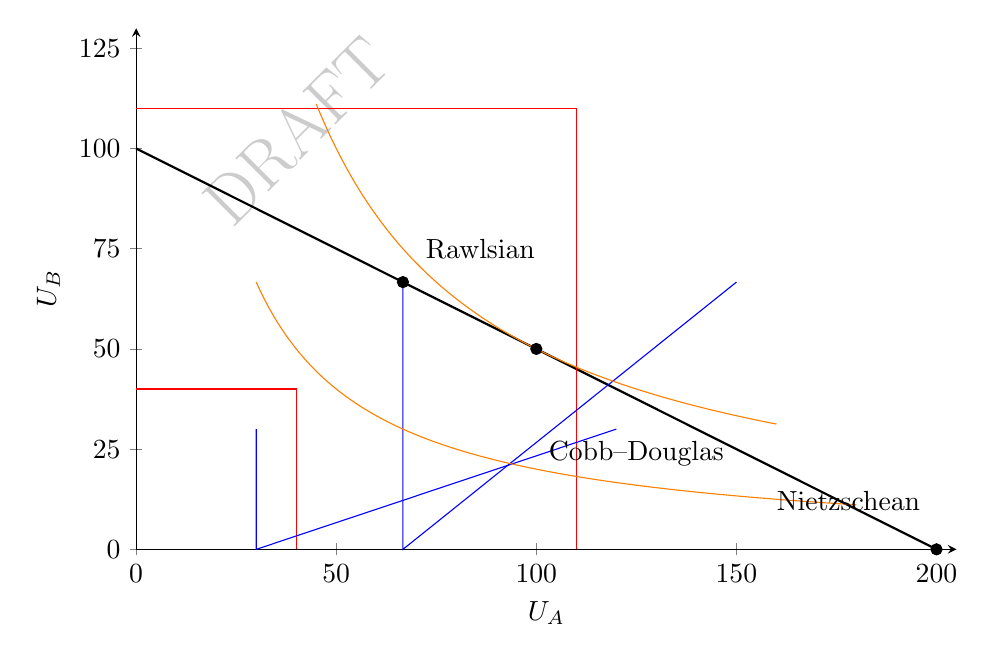
\begin{tikzpicture}
    \begin{axis}[
        width=12cm,
        height=8.2cm,
        xmin=0,xmax=205,
        ymin=0,ymax=130,
        axis lines=left,
        xlabel={$U_A$},
        ylabel={$U_B$},
        xtick={0,50,100,150,200},
        ytick={0,25,50,75,100,125},
        clip=false
    ]
    % frontier
    \addplot[domain=0:200,samples=2,thick,black] {100-0.5*x};

    % Nietzschean iso-welfare
    \addplot[red] coordinates {(40,0) (40,40) (0,40)};
    \addplot[red] coordinates {(110,0) (110,110) (0,110)};

    % Rawlsian iso-welfare
    \addplot[blue] coordinates {(30,30) (30,0) (120,30)};
    \addplot[blue] coordinates {(200/3,200/3) (200/3,0) (150,200/3)};

    % Cobb-Douglas isowelfare curves
    \addplot[orange,domain=30:180,samples=200] {2000/x};
    \addplot[orange,domain=45:160,samples=200] {5000/x};

    % points
    \addplot[only marks,mark=*,mark size=2pt] coordinates {(200,0) (200/3,200/3) (100,50)};
    \node at (axis cs:178,12) {Nietzschean};
    \node at (axis cs:86,75) {Rawlsian};
    \node at (axis cs:125,24) {Cobb--Douglas};
    \end{axis}
    \end{tikzpicture}
    \end{center}
\end{enumerate}

\subsubsection{Method 2: Slope matching and direct objective analysis}

\begin{enumerate}[label=(\alph*)]
    \item
    From
    \[
    U_A+2U_B=200,
    \]
    implicit differentiation gives
    \[
    1+2\frac{dU_B}{dU_A}=0
    \qquad\Longrightarrow\qquad
    \frac{dU_B}{dU_A}=-\frac12.
    \]
    So the frontier is a straight line of slope $-1/2$ with intercepts $(200,0)$ and $(0,100)$.

    \item
    For $W(U_A,U_B)=\max\{U_A,U_B\}$, the greatest possible welfare is obtained by making the larger of the two utilities as large as possible. Along the frontier the maximum achievable utility for person $A$ is 200, whereas for person $B$ it is only 100. Therefore the welfare-maximizing point is
    \[
    \boxed{(U_A,U_B)=(200,0).}
    \]

    \item
    For $W(U_A,U_B)=\min\{U_A,U_B\}$, the welfare level equals the smaller of the two utilities. The maximum of the minimum occurs where the two utilities are equal, because otherwise one could raise the smaller one without lowering the larger below it until equality is reached. Thus impose
    \[
    U_A=U_B.
    \]
    Combining with the frontier gives
    \[
    3U_A=200,
    \qquad
    U_A=U_B=\frac{200}{3}.
    \]
    Hence
    \[
    \boxed{\left(U_A,U_B\right)=\left(\frac{200}{3},\frac{200}{3}\right).}
    \]

    \item
    For
    \[
    W(U_A,U_B)=U_A^{1/2}U_B^{1/2},
    \]
    an isowelfare curve satisfies
    \[
    U_A^{1/2}U_B^{1/2}=\bar W.
    \]
    Taking logs or differentiating directly,
    \[
    \frac{dU_B}{dU_A}=-\frac{U_B}{U_A}
    \]
    along an isowelfare curve.

    At an interior optimum, the slope of the isowelfare curve equals the slope of the frontier:
    \[
    -\frac{U_B}{U_A}=-\frac12.
    \]
    Hence
    \[
    U_A=2U_B.
    \]
    Substitute into the frontier:
    \[
    2U_B+2U_B=200
    \qquad\Longrightarrow\qquad
    4U_B=200
    \qquad\Longrightarrow\qquad
    U_B=50.
    \]
    Therefore
    \[
    U_A=100.
    \]
    So the optimum is
    \[
    \boxed{(U_A,U_B)=(100,50).}
    \]
\end{enumerate}

\newpage
\subsection{ Question 1}
\subsubsection{Solution}

There are three policies \(X,Y,Z\), and three preference types:

\[
\text{Young: } Z \succ Y \succ X,
\qquad
\text{Middle Aged: } X \succ Z \succ Y,
\qquad
\text{Old: } Y \succ X \succ Z.
\]

The numbers of voters are:
\[
300 \text{ young}, \qquad 300 \text{ middle aged}, \qquad 400 \text{ old}.
\]

Under \emph{standard Borda voting} with three alternatives, each voter awards:
\[
\text{1st place } = 2 \text{ points}, 
\qquad
\text{2nd place } = 1 \text{ point}, 
\qquad
\text{3rd place } = 0 \text{ points}.
\]

Under the \emph{modified Borda voting} rule, the same ranking scores apply, except:
\begin{itemize}
    \item young voters' points are multiplied by \(2\),
    \item middle-aged voters' points are multiplied by \(1.5\),
    \item old voters' points remain unchanged.
\end{itemize}

\begin{enumerate}[label=(\alph*)]
    \item
    In general, the modified Borda rule gives \emph{more weight} to the preferences of young and middle-aged consumers, relative to old consumers.

    Under standard Borda, each person's ranking contributes equally. Under the modified rule:
    \[
    \text{Young weight }=2,
    \qquad
    \text{Middle-aged weight }=1.5,
    \qquad
    \text{Old weight }=1.
    \]
    So the social ranking will tend to shift toward alternatives that are ranked highly by the young and middle-aged groups, and away from alternatives that are mainly supported by the old group.

    In this problem:
    \begin{itemize}
        \item the young rank \(Z\) first,
        \item the middle-aged rank \(X\) first,
        \item the old rank \(Y\) first.
    \end{itemize}

    Hence, compared with standard Borda voting:
    \begin{itemize}
        \item \(Z\) should gain because the young are heavily up-weighted,
        \item \(X\) should also gain because the middle-aged are up-weighted,
        \item \(Y\) is likely to lose relative ground because the old group is not up-weighted.
    \end{itemize}

    So, \emph{in general}, the modified rule tilts the social ranking in favour of the policies preferred by the young and middle-aged, especially the young.

    \item
    Yes, the modified Borda voting rule satisfies the \emph{Pareto condition}.

    Recall the Pareto condition: if \emph{every} individual strictly prefers policy \(A\) to policy \(B\), then the social ranking must also place \(A\) above \(B\).

    Under Borda scoring with three alternatives, each voter gives more points to a higher-ranked alternative than to a lower-ranked one. So if every voter ranks \(A\) above \(B\), then for every voter,
    \[
    \text{score of }A > \text{score of }B.
    \]
    Under the modified rule, these individual scores are multiplied by positive weights (\(2\), \(1.5\), and \(1\)). Since all these weights are strictly positive, the inequality is preserved:
    \[
    \text{weighted score of }A > \text{weighted score of }B
    \]
    for every voter.

    Summing across all voters, the total weighted Borda score of \(A\) must exceed that of \(B\). Therefore the social ranking also places \(A\) above \(B\).

    Hence:
    \[
    \boxed{\text{The modified Borda rule satisfies the Pareto condition.}}
    \]

    \item
    We now compute the winning policy under the two voting rules.

    \textbf{(i) Standard Borda voting}

    Using the standard \(2,1,0\) scoring rule:

    \begin{center}
    \begin{tabular}{c|ccc}
    \toprule
    Group & First & Second & Third\\
    \midrule
    Young (\(300\)) & \(Z\) & \(Y\) & \(X\)\\
    Middle Aged (\(300\)) & \(X\) & \(Z\) & \(Y\)\\
    Old (\(400\)) & \(Y\) & \(X\) & \(Z\)\\
    \bottomrule
    \end{tabular}
    \end{center}

    Compute total scores:

    \[
    \begin{aligned}
    \text{Score}(X)
    &=300(0)+300(2)+400(1) \\
    &=0+600+400 \\
    &=1000,
    \end{aligned}
    \]

    \[
    \begin{aligned}
    \text{Score}(Y)
    &=300(1)+300(0)+400(2) \\
    &=300+0+800 \\
    &=1100,
    \end{aligned}
    \]

    \[
    \begin{aligned}
    \text{Score}(Z)
    &=300(2)+300(1)+400(0) \\
    &=600+300+0 \\
    &=900.
    \end{aligned}
    \]

    Therefore the standard Borda social ranking is
    \[
    Y \succ X \succ Z.
    \]
    So the chosen policy is
    \[
    \boxed{Y.}
    \]

    \bigskip

    \textbf{(ii) Modified Borda voting}

    Under the modified rule:
    \begin{itemize}
        \item young scores are multiplied by \(2\),
        \item middle-aged scores are multiplied by \(1.5\),
        \item old scores are unchanged.
    \end{itemize}

    So the effective contributions are:

    \[
    \begin{aligned}
    \text{Young contribution:}&\quad
    Z: 300(2)(2)=1200,\quad
    Y: 300(1)(2)=600,\quad
    X: 300(0)(2)=0.
    \end{aligned}
    \]

    \[
    \begin{aligned}
    \text{Middle-aged contribution:}\quad
    &X: 300(2)(1.5)=900,\quad Z: 300(1)(1.5)=450,\\
    &Y: 300(0)(1.5)=0.
    \end{aligned}
    \]

    \[
    \begin{aligned}
    \text{Old contribution:}&\quad
    Y: 400(2)=800,\quad
    X: 400(1)=400,\quad
    Z: 400(0)=0.
    \end{aligned}
    \]

    Summing up:

    \[
    \begin{aligned}
    \text{Modified Score}(X)&=0+900+400=1300,\\
    \text{Modified Score}(Y)&=600+0+800=1400,\\
    \text{Modified Score}(Z)&=1200+450+0=1650.
    \end{aligned}
    \]

    Therefore the modified Borda social ranking is
    \[
    Z \succ Y \succ X.
    \]
    So the chosen policy is
    \[
    \boxed{Z.}
    \]

    Hence:
    \[
    \boxed{\text{Standard Borda chooses }Y,\qquad \text{Modified Borda chooses }Z.}
    \]

    \item
    A reasonable argument in favour of the modified Borda rule is that environmental policy has \emph{long-term consequences}, so it may be appropriate to give greater weight to groups who will live with those consequences for longer.

    In this scenario:
    \begin{itemize}
        \item young consumers are likely to be affected by climate and environmental outcomes over a longer remaining lifetime,
        \item middle-aged consumers also have substantial future exposure, and may additionally care about their children,
        \item old consumers may be affected for a shorter period.
    \end{itemize}

    Under standard Borda voting, each person has the same weight, regardless of how long they will experience the effects of the policy. The modified rule instead places more emphasis on the preferences of those with a longer future stake in the consequences of environmental policy.

    So one may argue that the modified rule is more ``reasonable'' because it better reflects:
    \begin{itemize}
        \item intergenerational fairness,
        \item the long-run nature of environmental policy,
        \item the idea that those more affected by future outcomes should have greater influence.
    \end{itemize}

    However, this is a normative judgment rather than a purely mathematical one. A criticism is that it violates the principle of \emph{equal political weight} or ``one person, one vote.'' So whether it is more reasonable depends on the ethical criterion being used.

    A balanced conclusion is therefore:
    \begin{center}
    \fbox{\parbox{0.9\linewidth}{\centering
    The modified rule may be more reasonable if voting power should reflect long-run stakes in environmental outcomes, but less reasonable if every voter should have equal weight.
    }}
    \end{center}
\end{enumerate}

\newpage
\subsection{Question 2}
\subsubsection{Solution}

The utility possibility frontier (UPF) is given by
\[
U_I + U_J^2 = 10.
\]

We assume utilities are non-negative, so the relevant part of the frontier is
\[
U_I \ge 0,\qquad U_J \ge 0.
\]

\begin{enumerate}[label=(\alph*)]
    \item
    The \emph{utility possibility frontier} is the boundary of all utility pairs \((U_I,U_J)\) that can be achieved in the economy when resources are allocated efficiently.

    In other words:
    \begin{itemize}
        \item the set of feasible utility allocations gives all utility pairs the economy can generate,
        \item the \emph{frontier} consists of the Pareto efficient utility pairs,
        \item at a point on the frontier, one person's utility can be increased only by decreasing the other person's utility.
    \end{itemize}

    Since
    \[
    U_I + U_J^2 = 10,
    \]
    we can write the frontier as
    \[
    U_I = 10 - U_J^2
    \]
    or equivalently
    \[
    U_J = \sqrt{10-U_I}.
    \]

    The intercepts are:
    \[
    U_J=0 \implies U_I=10,
    \qquad
    U_I=0 \implies U_J=\sqrt{10}.
    \]

    So the UPF is downward sloping and bowed toward the origin in the \((U_I,U_J)\)-diagram.

    A suitable graph is:

    \begin{center}
    \begin{tikzpicture}
    \begin{axis}[
        width=11.5cm,
        height=8cm,
        xmin=0,xmax=10.5,
        ymin=0,ymax=3.6,
        axis lines=left,
        xlabel={$U_I$},
        ylabel={$U_J$},
        xtick={0,1,39/4,10},
        xticklabels={$0$,$1$,$\frac{39}{4}$,$10$},
        ytick={0,1/2,3,sqrt(10)},
        yticklabels={$0$,$\frac12$,$3$,$\sqrt{10}$},
        samples=200,
        domain=0:10,
        clip=false
    ]
    \addplot[thick,blue] {sqrt(10-x)};
    \addplot[dashed] coordinates {(1,0) (1,3)};
    \addplot[dashed] coordinates {(0,3) (1,3)};
    \addplot[dashed] coordinates {(39/4,0) (39/4,1/2)};
    \addplot[dashed] coordinates {(0,1/2) (39/4,1/2)};
    \addplot[only marks,mark=*,mark size=2pt] coordinates {(1,3) (39/4,1/2)};
    \node[blue] at (axis cs:7.9,2.1) {UPF: $U_J=\sqrt{10-U_I}$};
    \node at (axis cs:1.5,3.18) {$(1,3)$};
    \node at (axis cs:8.5,0.72) {$\left(\frac{39}{4},\frac12\right)$};
    \end{axis}
    \end{tikzpicture}
    \end{center}

    The feasible utility set is the region on and below this frontier:
    \[
    U_I + U_J^2 \le 10.
    \]

    \item
    A utilitarian social planner maximizes the sum of utilities:
    \[
    W(U_I,U_J)=U_I+U_J.
    \]

    Since on the frontier
    \[
    U_I=10-U_J^2,
    \]
    substituting into the welfare function gives
    \[
    W(U_J)=10-U_J^2+U_J.
    \]

    Differentiate:
    \[
    \frac{dW}{dU_J}=-2U_J+1.
    \]
    Setting the first-order condition equal to zero,
    \[
    -2U_J+1=0
    \quad\Longrightarrow\quad
    U_J=\frac12.
    \]

    Since
    \[
    \frac{d^2W}{dU_J^2}=-2<0,
    \]
    this is indeed the welfare-maximizing point.

    Then
    \[
    U_I=10-\left(\frac12\right)^2
    =10-\frac14
    =\frac{39}{4}.
    \]

    Therefore the utilitarian planner's ideal allocation is
    \[
    \boxed{
    U_I^*=\frac{39}{4},
    \qquad
    U_J^*=\frac12.}
    \]

    Graphically, this is the point where the highest attainable social indifference line
    \[
    U_I+U_J=\bar W
    \]
    is tangent to the utility possibility frontier.

    \item
    A weighted-utilitarian social welfare function has the form
    \[
    W(U_I,U_J)=\alpha U_I+\beta U_J,
    \]
    where \(\alpha,\beta>0\).

    We are told that the planner's ideal allocation is
    \[
    U_I=1,\qquad U_J=3.
    \]
    First check that this point lies on the utility possibility frontier:
    \[
    1+3^2=1+9=10.
    \]
    So it is feasible and efficient.

    To find the weights, maximize
    \[
    W=\alpha U_I+\beta U_J
    \]
    subject to
    \[
    U_I=10-U_J^2.
    \]
    Substituting:
    \[
    W(U_J)=\alpha(10-U_J^2)+\beta U_J.
    \]
    Differentiate:
    \[
    \frac{dW}{dU_J}=-2\alpha U_J+\beta.
    \]
    Setting the first-order condition equal to zero,
    \[
    -2\alpha U_J+\beta=0.
    \]
    Since the optimum is required to occur at \(U_J=3\),
    \[
    -2\alpha(3)+\beta=0
    \quad\Longrightarrow\quad
    \beta=6\alpha.
    \]

    So the weights must satisfy
    \[
    \frac{\beta}{\alpha}=6.
    \]
    One convenient choice is
    \[
    \alpha=1,\qquad \beta=6.
    \]

    Hence an appropriate social welfare function is
    \[
    \boxed{W(U_I,U_J)=U_I+6U_J.}
    \]
    Any positive scalar multiple of this is equivalent, for example
    \[
    2U_I+12U_J,\qquad \frac16 U_I+U_J,
    \]
    and so on.

    Graphically, the planner's social indifference curves are straight lines
    \[
    U_I+6U_J=\bar W
    \]
    or equivalently
    \[
    U_J=\frac{\bar W}{6}-\frac{1}{6}U_I,
    \]
    with slope
    \[
    -\frac{1}{6}.
    \]
    This matches the slope of the utility possibility frontier at \((1,3)\), confirming tangency there.

    Therefore:
    \[
    \boxed{\text{An appropriate weighted-utilitarian SWF is }W(U_I,U_J)=U_I+6U_J.}
    \]

    \item
    Not every point on the utility possibility frontier will necessarily be achievable as a competitive equilibrium \emph{from a given initial endowment}.

    The important ideas are:
    \begin{itemize}
        \item Every competitive equilibrium allocation is Pareto efficient under the standard assumptions. This is the \emph{First Welfare Theorem}.
        \item But the converse is more subtle. A Pareto efficient allocation need not arise as a competitive equilibrium for the \emph{current} initial endowment.
        \item However, under the standard convexity assumptions, every Pareto efficient allocation can be supported as a competitive equilibrium for \emph{some} redistribution of initial endowments. This is the \emph{Second Welfare Theorem}.
    \end{itemize}

    Therefore the correct discussion is:

    \begin{itemize}
        \item If the initial endowment is fixed, then \emph{not every} point on the UPF will generally be obtained as a competitive equilibrium.
        \item If the planner is allowed to redistribute endowments appropriately first, and if the economy satisfies the standard assumptions (convex preferences, local nonsatiation, etc.), then every point on the UPF can be decentralized as a competitive equilibrium.
    \end{itemize}

    So the best conclusion is:
    \begin{center}
    \fbox{\parbox{0.9\linewidth}{\centering
    Not necessarily for a fixed endowment, but under the standard assumptions every point on the UPF can be supported as a competitive equilibrium after a suitable redistribution of endowments.
    }}
    \end{center}
\end{enumerate}

% ============================================================
% QUESTION 1
% ============================================================

\newpage
\section{Sample Question 1: Weighted Borda Voting}

\subsection{Problem}

There are three policies \(X,Y,Z\), and three preference types:

\[
\text{Young: } Z \succ Y \succ X,
\qquad
\text{Middle Aged: } X \succ Z \succ Y,
\qquad
\text{Old: } Y \succ X \succ Z.
\]

The numbers of voters are:
\[
300 \text{ young}, \qquad 300 \text{ middle aged}, \qquad 400 \text{ old}.
\]

Under \emph{standard Borda voting} with three alternatives, each voter awards:
\[
\text{1st place } = 2 \text{ points}, 
\qquad
\text{2nd place } = 1 \text{ point}, 
\qquad
\text{3rd place } = 0 \text{ points}.
\]

Under the \emph{modified Borda voting} rule, the same ranking scores apply, except:
\begin{itemize}[leftmargin=*]
    \item young voters' points are multiplied by \(2\),
    \item middle-aged voters' points are multiplied by \(1.5\),
    \item old voters' points remain unchanged.
\end{itemize}

\begin{enumerate}[label=(\alph*)]
    \item In general, would the modified Borda voting rule make the social decision tend to align more with the old, the middle-aged, or the young? Explain briefly.
    \item Does the modified Borda voting rule satisfy the Pareto condition? Explain briefly.
    \item Which policy would be chosen under the standard Borda voting rule, and which policy would be chosen under the modified Borda voting rule?
    \item Do you think the modified Borda voting rule is more reasonable in this environmental policy context? Briefly explain.
\end{enumerate}

\newpage

\subsection{Solution}

\subsubsection{Method 1: Direct weighted-score computation}

\begin{enumerate}[label=(\alph*)]
    \item
    In general, the modified Borda rule gives more weight to the preferences of young and middle-aged consumers relative to old consumers.

    Under standard Borda, each person's ranking contributes equally. Under the modified rule:
    \[
    \text{Young weight }=2,
    \qquad
    \text{Middle-aged weight }=1.5,
    \qquad
    \text{Old weight }=1.
    \]
    So the social ranking will tend to shift toward alternatives that are ranked highly by the young and middle-aged groups, and away from alternatives that are mainly supported by the old group.

    In this problem:
    \begin{itemize}[leftmargin=*]
        \item the young rank \(Z\) first,
        \item the middle-aged rank \(X\) first,
        \item the old rank \(Y\) first.
    \end{itemize}

    Hence, compared with standard Borda voting:
    \begin{itemize}[leftmargin=*]
        \item \(Z\) should gain because the young are heavily up-weighted,
        \item \(X\) should also gain because the middle-aged are up-weighted,
        \item \(Y\) is likely to lose relative ground because the old group is not up-weighted.
    \end{itemize}

    Therefore
    \begin{center}
    \fbox{\parbox{0.9\linewidth}{\centering
    The modified rule tends to align more with the young and middle-aged, especially the young.
    }}
    \end{center}

    \item
    Yes, the modified Borda voting rule satisfies the Pareto condition.

    If every individual strictly prefers policy \(A\) to policy \(B\), then under ordinary Borda scoring each person assigns strictly more points to \(A\) than to \(B\). Under the modified rule, these scores are multiplied by strictly positive weights \(2\), \(1.5\), and \(1\), so the strict inequality is preserved for every voter.

    Summing across all voters, the total weighted Borda score of \(A\) must exceed that of \(B\). Therefore the social ranking also places \(A\) above \(B\).

    Hence
    \[
    \boxed{\text{the modified Borda rule satisfies the Pareto condition.}}
    \]

    \item
    \textbf{Standard Borda voting.}

    The three groups rank:
    \[
    \text{Young: } Z \succ Y \succ X,
    \qquad
    \text{Middle Aged: } X \succ Z \succ Y,
    \qquad
    \text{Old: } Y \succ X \succ Z.
    \]

    Using the standard \(2,1,0\) scoring rule:
    \[
    \begin{aligned}
    \text{Score}(X)
    &=300(0)+300(2)+400(1)=1000,\\
    \text{Score}(Y)
    &=300(1)+300(0)+400(2)=1100,\\
    \text{Score}(Z)
    &=300(2)+300(1)+400(0)=900.
    \end{aligned}
    \]
    Therefore the standard Borda social ranking is
    \[
    Y \succ X \succ Z,
    \]
    so the chosen policy is
    \[
    \boxed{Y.}
    \]

    \bigskip

    \textbf{Modified Borda voting.}

    Under the modified rule:
    \begin{itemize}[leftmargin=*]
        \item young scores are multiplied by \(2\),
        \item middle-aged scores are multiplied by \(1.5\),
        \item old scores are unchanged.
    \end{itemize}

    So the weighted contributions are:
    \[
    \begin{aligned}
    \text{Modified Score}(X)
    &=300(0)(2)+300(2)(1.5)+400(1)(1)\\
    &=0+900+400=1300,\\
    \text{Modified Score}(Y)
    &=300(1)(2)+300(0)(1.5)+400(2)(1)\\
    &=600+0+800=1400,\\
    \text{Modified Score}(Z)
    &=300(2)(2)+300(1)(1.5)+400(0)(1)\\
    &=1200+450+0=1650.
    \end{aligned}
    \]
    Therefore the modified Borda social ranking is
    \[
    Z \succ Y \succ X,
    \]
    so the chosen policy is
    \[
    \boxed{Z.}
    \]

    Hence
    \[
    \boxed{\text{Standard Borda chooses }Y,\qquad \text{Modified Borda chooses }Z.}
    \]

    \item
    A reasonable argument in favour of the modified Borda rule is that environmental policy has long-term consequences, so it may be appropriate to give greater weight to groups who will live with those consequences for longer.

    In this scenario:
    \begin{itemize}[leftmargin=*]
        \item young consumers are likely to be affected by environmental outcomes over a longer remaining lifetime,
        \item middle-aged consumers also have substantial future exposure,
        \item old consumers may be affected for a shorter period.
    \end{itemize}

    Under standard Borda voting, each person has the same weight regardless of how long they will experience the effects of the policy. The modified rule instead places more emphasis on the preferences of those with a longer future stake.

    A criticism, however, is that it violates the principle of equal political weight or ``one person, one vote.'' So whether it is more reasonable depends on the ethical principle being used.

    A balanced conclusion is:
    \begin{center}
    \fbox{\parbox{0.9\linewidth}{\centering
    The modified rule may be more reasonable if voting power should reflect long-run stakes in environmental outcomes, but less reasonable if every voter should have equal weight.
    }}
    \end{center}
\end{enumerate}

\subsubsection{Method 2: Linear-functional / vector method}

\begin{enumerate}[label=(\alph*)]
    \item
    Write the standard Borda score vector for \((\text{1st},\text{2nd},\text{3rd})\) as
    \[
    s=(2,1,0).
    \]
    The modified rule is simply a reweighting of group contributions by
    \[
    w=(2,1.5,1).
    \]
    Since the young and middle-aged groups are upweighted relative to the old group, the induced social ranking shifts toward the alternatives they rank highly. Since the young place \(Z\) first and the middle-aged place \(X\) first, while the old place \(Y\) first, the modified rule moves weight away from \(Y\) and toward \(Z\) and \(X\), especially \(Z\).

    \item
    The Pareto condition follows immediately from positivity of the weights. If every voter ranks \(A\) above \(B\), then every group contributes a strictly larger Borda score to \(A\) than to \(B\). Multiplying by positive weights preserves the inequality, so total weighted score still ranks \(A\) above \(B\).

    \item
    Let the score vector for each policy under the three groups be:
    \[
    X=(0,2,1),\qquad Y=(1,0,2),\qquad Z=(2,1,0).
    \]
    Under standard Borda, with population vector
    \[
    n=(300,300,400),
    \]
    the total scores are proportional to
    \[
    \langle n,X\rangle =1000,\qquad
    \langle n,Y\rangle =1100,\qquad
    \langle n,Z\rangle =900.
    \]
    Hence
    \[
    \boxed{Y \succ X \succ Z.}
    \]

    Under modified Borda, the effective population vector is
    \[
    n'=(600,450,400),
    \]
    so
    \[
    \langle n',X\rangle =1300,\qquad
    \langle n',Y\rangle =1400,\qquad
    \langle n',Z\rangle =1650.
    \]
    Hence
    \[
    \boxed{Z \succ Y \succ X.}
    \]

    Therefore standard Borda chooses \(Y\) and modified Borda chooses \(Z\).

    \item
    In this representation, the modified rule changes the social ranking by changing the weight vector. So the normative question is whether one regards this change of weight vector as ethically justified. If voting weight should reflect future stake, the modification is defensible; if all persons should count equally, it is not.
\end{enumerate}

\newpage
\subsubsection{Method 3: Pairwise score-difference method}

\begin{enumerate}[label=(\alph*)]
    \item
    Under the modified rule, the relative influence of the young and middle-aged groups rises, while the old group keeps weight 1. Therefore alternatives favoured by the young and middle-aged gain relative to alternatives favoured mainly by the old.

    \item
    If everyone ranks \(A\) above \(B\), then each individual contributes a strictly higher Borda score to \(A\) than to \(B\). Positive reweighting preserves this group-by-group advantage, so the aggregate ranking still has \(A\) above \(B\). Thus Pareto holds.

    \item
    Instead of computing all totals, compare relevant score differences.

    Under standard Borda:
    \[
    \begin{aligned}
    \text{Score}(Y)-\text{Score}(X)
    &=300(1-0)+300(0-2)+400(2-1)\\
    &=300-600+400=100>0,
    \end{aligned}
    \]
    so \(Y\succ X\).

    Also,
    \[
    \begin{aligned}
    \text{Score}(X)-\text{Score}(Z)
    &=300(0-2)+300(2-1)+400(1-0)\\
    &=-600+300+400=100>0,
    \end{aligned}
    \]
    so \(X\succ Z\). Hence
    \[
    \boxed{Y \succ X \succ Z.}
    \]

    Under modified Borda:
    \[
    \begin{aligned}
    \text{Score}(Z)-\text{Score}(Y)
    &=300\cdot 2(2-1)+300\cdot 1.5(1-0)+400\cdot 1(0-2)\\
    &=600+450-800=250>0,
    \end{aligned}
    \]
    so \(Z\succ Y\).

    Next,
    \[
    \begin{aligned}
    \text{Score}(Y)-\text{Score}(X)
    &=300\cdot 2(1-0)+300\cdot 1.5(0-2)+400\cdot 1(2-1)\\
    &=600-900+400=100>0,
    \end{aligned}
    \]
    so \(Y\succ X\). Hence
    \[
    \boxed{Z \succ Y \succ X.}
    \]

    \item
    Since the modified rule makes \(Z\) overtake \(Y\) precisely because of the heavier weight placed on the young and middle-aged, the reasonableness of the rule depends on whether that reweighting is normatively acceptable.
\end{enumerate}
\newpage\subsubsection{Marking scheme (20 marks)}

\begin{enumerate}[label=(\alph*)]
    \item \textbf{(4 marks)} Comparative effect of the modified weights
    \begin{itemize}[leftmargin=*]
        \item 2 marks: Correct identification that the modified rule shifts influence toward the young and middle-aged, especially the young.
        \item 2 marks: Clear explanation using the weight changes \(2,1.5,1\) and the ranking pattern of the three groups.
    \end{itemize}

    \item \textbf{(4 marks)} Pareto condition
    \begin{itemize}[leftmargin=*]
        \item 2 marks: Correct conclusion that the modified Borda rule satisfies the Pareto condition.
        \item 2 marks: Correct justification that positive weighting preserves the strict score advantage of a unanimously preferred alternative.
    \end{itemize}

    \item \textbf{(8 marks)} Policy choice under standard and modified Borda
    \begin{itemize}[leftmargin=*]
        \item 3 marks: Correct standard Borda score calculation or an equivalent correct derivation.
        \item 3 marks: Correct modified Borda score calculation or an equivalent correct derivation.
        \item 2 marks: Correct final conclusion that standard Borda chooses \(Y\) while modified Borda chooses \(Z\).
    \end{itemize}

    \item \textbf{(4 marks)} Reasonableness in context
    \begin{itemize}[leftmargin=*]
        \item 2 marks: A coherent argument in favour of the modified rule based on long-run stake / intergenerational exposure.
        \item 2 marks: Recognition of the counterargument concerning equal political weight, together with a balanced conclusion.
    \end{itemize}
\end{enumerate}
% ============================================================
% QUESTION 2
% ============================================================

\newpage
\section{Sample Question 2: Utility Possibility Frontier and Welfare Optimisation}

\subsection{Problem}

The utility possibility frontier (UPF) is given by
\[
U_I + U_J^2 = 10.
\]

We assume utilities are non-negative, so the relevant part of the frontier is
\[
U_I \ge 0,\qquad U_J \ge 0.
\]

\begin{enumerate}[label=(\alph*)]
    \item Explain what the utility possibility frontier means, and sketch it in the \((U_I,U_J)\)-plane.
    \item If a utilitarian social planner maximizes
    \[
    W(U_I,U_J)=U_I+U_J,
    \]
    what is the planner's ideal allocation?
    \item If a weighted-utilitarian social welfare function is used, and the planner's ideal allocation is
    \[
    U_I=1,\qquad U_J=3,
    \]
    what weighted-utilitarian social welfare function would support this point?
    \item Is every point on the utility possibility frontier necessarily obtainable as a competitive equilibrium? Briefly explain.
\end{enumerate}

\newpage
\subsection{Solution}

\subsubsection{Method 1: Direct substitution and tangency}

\begin{enumerate}[label=(\alph*)]
    \item
    The \emph{utility possibility frontier} is the boundary of all utility pairs \((U_I,U_J)\) that can be achieved in the economy when resources are allocated efficiently.

    In other words:
    \begin{itemize}[leftmargin=*]
        \item the feasible utility set consists of all utility pairs the economy can generate,
        \item the \emph{frontier} consists of the Pareto efficient utility pairs,
        \item at a point on the frontier, one person's utility can be increased only by decreasing the other person's utility.
    \end{itemize}

    Since
    \[
    U_I + U_J^2 = 10,
    \]
    we can write the frontier as
    \[
    U_I = 10 - U_J^2
    \]
    or equivalently
    \[
    U_J = \sqrt{10-U_I}.
    \]

    The intercepts are:
    \[
    U_J=0 \implies U_I=10,
    \qquad
    U_I=0 \implies U_J=\sqrt{10}.
    \]
    So the UPF is downward sloping and bowed toward the origin in the \((U_I,U_J)\)-diagram, and the feasible set is
    \[
    \boxed{U_I+U_J^2\le 10.}
    \]
    A suitable graph is:

    \begin{center}
    \begin{tikzpicture}
    \begin{axis}[
        width=11.5cm,
        height=8cm,
        xmin=0,xmax=10.5,
        ymin=0,ymax=3.6,
        axis lines=left,
        xlabel={$U_I$},
        ylabel={$U_J$},
        xtick={0,1,39/4,10},
        xticklabels={$0$,$1$,$\frac{39}{4}$,$10$},
        ytick={0,1/2,3,sqrt(10)},
        yticklabels={$0$,$\frac12$,$3$,$\sqrt{10}$},
        samples=200,
        domain=0:10,
        clip=false
    ]
    \addplot[thick,blue] {sqrt(10-x)};
    \addplot[dashed] coordinates {(1,0) (1,3)};
    \addplot[dashed] coordinates {(0,3) (1,3)};
    \addplot[dashed] coordinates {(39/4,0) (39/4,1/2)};
    \addplot[dashed] coordinates {(0,1/2) (39/4,1/2)};
    \addplot[only marks,mark=*,mark size=2pt] coordinates {(1,3) (39/4,1/2)};
    \node[blue] at (axis cs:7.9,2.1) {UPF: $U_J=\sqrt{10-U_I}$};
    \node at (axis cs:1.5,3.18) {$(1,3)$};
    \node at (axis cs:8.5,0.72) {$\left(\frac{39}{4},\frac12\right)$};
    \end{axis}
    \end{tikzpicture}
    \end{center}
    \item
    A utilitarian social planner maximizes
    \[
    W(U_I,U_J)=U_I+U_J.
    \]
    Since on the frontier
    \[
    U_I=10-U_J^2,
    \]
    substitute into welfare:
    \[
    W(U_J)=10-U_J^2+U_J.
    \]
    Differentiate:
    \[
    \frac{dW}{dU_J}=-2U_J+1.
    \]
    Set equal to zero:
    \[
    -2U_J+1=0
    \quad\Longrightarrow\quad
    U_J=\frac12.
    \]
    Then
    \[
    U_I=10-\left(\frac12\right)^2=10-\frac14=\frac{39}{4}.
    \]
    Therefore the utilitarian optimum is
    \[
    \boxed{U_I^*=\frac{39}{4},\qquad U_J^*=\frac12.}
    \]

    \item
    A weighted-utilitarian social welfare function has the form
    \[
    W(U_I,U_J)=\alpha U_I+\beta U_J,
    \qquad \alpha,\beta>0.
    \]
    We are told that the ideal allocation is
    \[
    U_I=1,\qquad U_J=3.
    \]
    First check feasibility:
    \[
    1+3^2=10.
    \]
    So the point lies on the frontier.

    Substitute \(U_I=10-U_J^2\) into welfare:
    \[
    W(U_J)=\alpha(10-U_J^2)+\beta U_J.
    \]
    Differentiate:
    \[
    \frac{dW}{dU_J}=-2\alpha U_J+\beta.
    \]
    Set equal to zero at \(U_J=3\):
    \[
    -2\alpha(3)+\beta=0
    \quad\Longrightarrow\quad
    \beta=6\alpha.
    \]
    So the required weight ratio is
    \[
    \boxed{\frac{\beta}{\alpha}=6.}
    \]
    One valid supporting welfare function is
    \[
    \boxed{W(U_I,U_J)=U_I+6U_J.}
    \]

    \item
    Not every point on the utility possibility frontier is necessarily obtainable as a competitive equilibrium from a \emph{given} initial endowment.

    The relevant economic principles are:
    \begin{itemize}[leftmargin=*]
        \item The \emph{First Welfare Theorem}: every competitive equilibrium allocation is Pareto efficient under the usual assumptions.
        \item The \emph{Second Welfare Theorem}: under suitable convexity assumptions, every Pareto efficient allocation can be decentralised as a competitive equilibrium for \emph{some} suitable redistribution of endowments.
    \end{itemize}

    Therefore:
    \begin{center}
    \fbox{\parbox{0.9\linewidth}{\centering
    Not necessarily for a fixed endowment, but under the standard assumptions every point on the UPF can be supported as a competitive equilibrium after a suitable redistribution of endowments.
    }}
    \end{center}
\end{enumerate}

\newpage
\subsubsection{Method 2: Lagrangian method}

\begin{enumerate}[label=(\alph*)]
    \item
    The UPF is the boundary of the feasible utility set
    \[
    \{(U_I,U_J)\in \R_+^2: U_I+U_J^2\le 10\}.
    \]
    The frontier itself is
    \[
    U_I+U_J^2=10,
    \]
    with intercepts \((10,0)\) and \((0,\sqrt{10})\).

    \item
    Maximize
    \[
    U_I+U_J
    \]
    subject to
    \[
    U_I+U_J^2=10.
    \]
    The Lagrangian is
    \[
    \mathcal L = U_I+U_J+\lambda(10-U_I-U_J^2).
    \]
    First-order conditions:
    \begin{align*}
        \frac{\partial \mathcal L}{\partial U_I} &= 1-\lambda=0,\\
        \frac{\partial \mathcal L}{\partial U_J} &= 1-2\lambda U_J=0.
    \end{align*}
    From the first equation,
    \[
    \lambda=1.
    \]
    Substitute into the second:
    \[
    1-2U_J=0
    \quad\Longrightarrow\quad
    U_J=\frac12.
    \]
    Then
    \[
    U_I=10-\left(\frac12\right)^2=\frac{39}{4}.
    \]
    Hence
    \[
    \boxed{\left(U_I^*,U_J^*\right)=\left(\frac{39}{4},\frac12\right).}
    \]
\newpage
    \item
    Now maximize
    \[
    \alpha U_I+\beta U_J
    \]
    subject to
    \[
    U_I+U_J^2=10.
    \]
    The Lagrangian is
    \[
    \mathcal L = \alpha U_I+\beta U_J+\lambda(10-U_I-U_J^2).
    \]
    FOCs:
    \begin{align*}
        \alpha-\lambda &=0,\\
        \beta-2\lambda U_J &=0.
    \end{align*}
    Hence
    \[
    \lambda=\alpha,
    \qquad
    \beta=2\alpha U_J.
    \]
    At the required point \(U_J=3\),
    \[
    \beta=6\alpha.
    \]
    Therefore
    \[
    \boxed{\frac{\beta}{\alpha}=6,}
    \]
    and one valid welfare function is
    \[
    \boxed{W(U_I,U_J)=U_I+6U_J.}
    \]

    \item
    The Lagrangian analysis solves a planner's problem, not necessarily a competitive-equilibrium problem for a fixed endowment. Competitive equilibrium requires decentralisation from a specific wealth distribution. Thus a point may be planner-efficient without being a competitive equilibrium for the original endowment vector. With appropriate redistribution and the standard assumptions, however, the Second Welfare Theorem allows decentralisation of every Pareto efficient point.
\end{enumerate}

\newpage
\subsubsection{Method 3: Convex-analysis / supporting-hyperplane method}

\begin{enumerate}[label=(\alph*)]
    \item
    Define the feasible utility set
    \[
    \mathcal U=\{(U_I,U_J)\in \R_+^2: U_I+U_J^2\le 10\}.
    \]
    Since \(U_J^2\) is convex, the set \(\mathcal U\) is convex. Its boundary
    \[
    U_I+U_J^2=10
    \]
    is the utility possibility frontier.

    \item
    The utilitarian planner maximizes the linear functional
    \[
    (U_I,U_J)\mapsto U_I+U_J
    \]
    over the convex set \(\mathcal U\). Therefore the optimum is the point on the boundary where the supporting line with normal vector \((1,1)\) touches the frontier.

    The frontier is the zero set of
    \[
    F(U_I,U_J)=U_I+U_J^2-10.
    \]
    Its normal vector is
    \[
    \nabla F=(1,2U_J).
    \]
    At a supporting point for utilitarian welfare, the normal vector to the frontier must be parallel to the normal vector of the welfare level sets, namely \((1,1)\). So
    \[
    (1,2U_J)\parallel (1,1).
    \]
    Hence
    \[
    2U_J=1
    \quad\Longrightarrow\quad
    U_J=\frac12.
    \]
    Therefore
    \[
    U_I=10-\frac14=\frac{39}{4}.
    \]
    Thus
    \[
    \boxed{\left(U_I^*,U_J^*\right)=\left(\frac{39}{4},\frac12\right).}
    \]

    \item
    For weighted-utilitarian welfare
    \[
    W(U_I,U_J)=\alpha U_I+\beta U_J,
    \]
    the supporting hyperplanes have normal vector
    \[
    (\alpha,\beta).
    \]
    At \((1,3)\), the frontier normal vector is
    \[
    \nabla F(1,3)=(1,6).
    \]
    Therefore the supporting welfare weights must satisfy
    \[
    (\alpha,\beta)\parallel (1,6).
    \]
    So
    \[
    \boxed{\frac{\beta}{\alpha}=6,}
    \]
    and one valid welfare function is
    \[
    \boxed{W(U_I,U_J)=U_I+6U_J.}
    \]

    \item
    The convex-analysis perspective makes the decentralisation issue transparent: competitive equilibria correspond to support by price hyperplanes from a given endowment, whereas Pareto efficient points are merely supportable boundary points of the feasible utility set. Thus supportability by a planner's welfare functional is weaker than supportability by competitive equilibrium from a fixed initial allocation.
\end{enumerate}

\newpage
\subsubsection{Method 4: Duality / planner-support method}

\begin{enumerate}[label=(\alph*)]
    \item
    The UPF is the \emph{primal} efficient boundary
    \[
    U_I+U_J^2=10
    \]
    of the feasible utility set. The planner's welfare problem is the corresponding \emph{dual support problem}: choose a linear welfare functional whose highest attainable indifference line touches the frontier.

    \item
    For utilitarian welfare
    \[
    W(U_I,U_J)=U_I+U_J,
    \]
    the dual problem is
    \[
    \max\{U_I+U_J: U_I+U_J^2\le 10\}.
    \]
    The support line has slope \(-1\). The frontier has slope
    \[
    \frac{dU_I}{dU_J}=-2U_J.
    \]
    Dual optimality requires equality of slopes:
    \[
    -2U_J=-1.
    \]
    Hence
    \[
    U_J=\frac12,\qquad U_I=\frac{39}{4}.
    \]
    Therefore
    \[
    \boxed{\left(U_I^*,U_J^*\right)=\left(\frac{39}{4},\frac12\right).}
    \]

    \item
    If a point \((1,3)\) is to be planner-optimal under a weighted-utilitarian functional, then the dual support line through that point must have the same slope as the frontier there. Since the frontier slope at \(U_J=3\) is
    \[
    -2U_J=-6,
    \]
    the welfare line
    \[
    \alpha U_I+\beta U_J=\bar W
    \]
    must have slope
    \[
    -\frac{\alpha}{\beta}=-\frac16
    \quad\Longrightarrow\quad
    \frac{\beta}{\alpha}=6.
    \]
    Thus
    \[
    \boxed{W(U_I,U_J)=U_I+6U_J}
    \]
    is a valid supporting welfare function.

    \item
    Duality also clarifies the equilibrium question. A planner's welfare function can support any efficient point by choosing an appropriate linear objective. Competitive equilibrium support is more restrictive: the supporting prices and wealth distribution must arise from market decentralisation. Therefore not every efficient point is a competitive equilibrium for a given initial endowment, although under the standard assumptions each efficient point can be decentralised after suitable redistribution.
\end{enumerate}

\newpage
\subsubsection{Marking scheme (20 marks)}

\begin{enumerate}[label=(\alph*)]
    \item \textbf{(5 marks)} Meaning and graph of the UPF
    \begin{itemize}[leftmargin=*]
        \item 2 marks: Correct explanation that the UPF is the set of Pareto efficient feasible utility allocations.
        \item 1 mark: Correct intercepts \((10,0)\) and \((0,\sqrt{10})\) or an equivalent correct characterisation.
        \item 2 marks: Correct sketch and correct description of the feasible set \(U_I+U_J^2\le 10\).
    \end{itemize}

    \item \textbf{(5 marks)} Utilitarian optimum
    \begin{itemize}[leftmargin=*]
        \item 2 marks: Correct optimisation setup.
        \item 2 marks: Correct solution \(\left(\frac{39}{4},\frac12\right)\).
        \item 1 mark: Correct justification that this is the maximiser.
    \end{itemize}

    \item \textbf{(5 marks)} Weighted-utilitarian support
    \begin{itemize}[leftmargin=*]
        \item 2 marks: Correct tangency / first-order condition linking weights to the slope at \((1,3)\).
        \item 2 marks: Correct weight ratio \(\beta/\alpha = 6\).
        \item 1 mark: A correct supporting welfare function, e.g. \(W(U_I,U_J)=U_I+6U_J\).
    \end{itemize}

    \item \textbf{(5 marks)} Competitive-equilibrium interpretation
    \begin{itemize}[leftmargin=*]
        \item 2 marks: Correct distinction between fixed endowment and redistributed endowment.
        \item 2 marks: Correct use of the First and / or Second Welfare Theorem.
        \item 1 mark: Clear final conclusion.
    \end{itemize}
\end{enumerate}


\end{document}
\newpage
\subsection{Utilitarianism Question 1}
\subsubsection{Solution}

Let \(x_A\) and \(x_B\) denote the amounts of good \(X\) allocated to consumers A and B respectively. Since the total endowment is \(100\), feasibility requires
\[
x_A+x_B=100,
\qquad
x_A\ge 0,\;x_B\ge 0.
\]

The utilities are
\[
U^A=x_A,
\qquad
U^B=\sqrt{x_B}.
\]

\begin{enumerate}[label=(\alph*)]
    \item
    We first consider the economy \emph{without} monetary transfers.

    An allocation \((x_A,x_B)\) is Pareto efficient if there is no other feasible allocation that makes one consumer strictly better off and the other at least as well off.

    Since both utility functions are strictly increasing in own consumption:
    \[
    \frac{dU^A}{dx_A}=1>0,
    \qquad
    \frac{dU^B}{dx_B}=\frac{1}{2\sqrt{x_B}}>0 \quad \text{for } x_B>0,
    \]
    each consumer always prefers more of good \(X\).

    Therefore:

    \begin{itemize}
        \item Any allocation with
        \[
        x_A+x_B<100
        \]
        cannot be Pareto efficient, because some unallocated units of \(X\) remain. Giving one of these extra units to either consumer would make that consumer strictly better off without making the other worse off.

        \item Any allocation with
        \[
        x_A+x_B=100
        \]
        is Pareto efficient. The reason is that to make A better off, we must increase \(x_A\), which necessarily reduces \(x_B\), making B worse off. Similarly, to make B better off, we must increase \(x_B\), which necessarily reduces \(x_A\), making A worse off.
    \end{itemize}

    Hence the set of Pareto efficient allocations is
    \[
    \boxed{
    \{(x_A,x_B): x_A+x_B=100,\; x_A\ge 0,\; x_B\ge 0\}.}
    \]

    So \emph{every} feasible allocation that exhausts the total endowment is Pareto efficient.

    \item
    A utilitarian allocation maximizes the sum of utilities:
    \[
    W(x_A,x_B)=U^A+U^B=x_A+\sqrt{x_B}
    \]
    subject to
    \[
    x_A+x_B=100.
    \]

    Substitute
    \[
    x_A=100-x_B.
    \]
    Then
    \[
    W(x_B)=100-x_B+\sqrt{x_B}.
    \]

    Differentiate:
    \[
    \frac{dW}{dx_B}=-1+\frac{1}{2\sqrt{x_B}}.
    \]
    Set the first-order condition equal to zero:
    \[
    -1+\frac{1}{2\sqrt{x_B}}=0
    \quad\Longrightarrow\quad
    \frac{1}{2\sqrt{x_B}}=1
    \quad\Longrightarrow\quad
    \sqrt{x_B}=\frac12
    \quad\Longrightarrow\quad
    x_B=\frac14.
    \]

    Since
    \[
    \frac{d^2W}{dx_B^2}
    =-\frac{1}{4x_B^{3/2}}<0 \quad \text{for }x_B>0,
    \]
    this gives the unique maximizer.

    Therefore
    \[
    x_B^*=\frac14,
    \qquad
    x_A^*=100-\frac14=\frac{399}{4}.
    \]

    So the utilitarian allocation is
    \[
    \boxed{
    \left(x_A^*,x_B^*\right)=\left(\frac{399}{4},\frac14\right).}
    \]

    \item
    Now suppose monetary transfers are allowed. Let the transfers be \(t^A\) and \(t^B\), with balanced budget:
    \[
    t^A+t^B=0.
    \]

    Utilities are quasi-linear in transfers:
    \[
    V^A=U^A+t^A=x_A+t^A,
    \qquad
    V^B=U^B+t^B=\sqrt{x_B}+t^B.
    \]

    A policy is now a pair
    \[
    \bigl((x_A,x_B),(t^A,t^B)\bigr)
    \]
    satisfying
    \[
    x_A+x_B=100,
    \qquad
    t^A+t^B=0.
    \]

    The key observation is that transfers only redistribute utility between the two consumers; they do not change the total:
    \[
    V^A+V^B
    =
    x_A+\sqrt{x_B}+t^A+t^B
    =
    x_A+\sqrt{x_B}.
    \]

    Therefore, with transfers available, Pareto efficiency requires the allocation of good \(X\) to maximize
    \[
    x_A+\sqrt{x_B}.
    \]
    But this is exactly the same objective as in part (b), so the Pareto efficient policies must allocate \(X\) in the utilitarian way:
    \[
    \boxed{
    x_A=\frac{399}{4},
    \qquad
    x_B=\frac14.}
    \]

    Compared with part (a), the answer changes sharply:

    \begin{itemize}
        \item \textbf{Without transfers:} every full allocation of \(X\) is Pareto efficient.
        \item \textbf{With transfers:} only the allocation
        \[
        \left(\frac{399}{4},\frac14\right)
        \]
        of good \(X\) can appear in a Pareto efficient policy.
    \end{itemize}

    The reason is that, once transfers are allowed, any loss suffered by one consumer from reallocating \(X\) can be compensated by a transfer, so efficiency boils down to maximizing total utility.

    \item
    Since all Pareto efficient policies must use the allocation
    \[
    \left(x_A,x_B\right)=\left(\frac{399}{4},\frac14\right),
    \]
    different Pareto efficient policies differ only in the transfer pair \((t^A,t^B)\), provided
    \[
    t^A+t^B=0.
    \]

    Two examples are:

    \[
    \boxed{
    \left(\frac{399}{4},\frac14,\;0,\;0\right)}
    \]
    and
    \[
    \boxed{
    \left(\frac{399}{4},\frac14,\;-5,\;5\right).}
    \]

    In the first example, there are no transfers. In the second, A pays \(5\) units of transfer to B. Both are Pareto efficient because they use the efficient allocation of good \(X\), and the transfers are balanced.
\end{enumerate}

\newpage
\subsection{Question 2}
\subsubsection{Solution}

We now prove the following statement:

\begin{quote}
If an allocation \(A\) is utilitarian, then there exists some transfer vector \(t\) such that the policy \((A,t)\) is Pareto efficient.
\end{quote}

In fact, we will prove a stronger statement: if \(A\) is utilitarian, then \emph{any} balanced transfer vector \(t\) makes \((A,t)\) Pareto efficient.

Let there be \(n\) consumers. For consumer \(i\), let gross utility from allocation \(A\) be \(U_i(A)\), and let total utility under transfers be
\[
V_i(A,t)=U_i(A)+t_i.
\]
Assume transfers are balanced:
\[
\sum_{i=1}^n t_i = 0.
\]

Suppose allocation \(A\) is utilitarian. This means that \(A\) maximizes the sum of gross utilities:
\[
\sum_{i=1}^n U_i(A)
\;\ge\;
\sum_{i=1}^n U_i(B)
\qquad
\text{for every feasible allocation } B.
\]

We claim that the policy \((A,t)\) is Pareto efficient for any balanced transfer vector \(t\).

Assume, for contradiction, that \((A,t)\) is \emph{not} Pareto efficient. Then there exists another feasible policy \((B,s)\) such that
\[
U_i(B)+s_i \ge U_i(A)+t_i
\qquad \text{for all }i,
\]
with strict inequality for at least one consumer \(j\):
\[
U_j(B)+s_j > U_j(A)+t_j.
\]

Summing across all consumers gives
\[
\sum_{i=1}^n \bigl(U_i(B)+s_i\bigr)
>
\sum_{i=1}^n \bigl(U_i(A)+t_i\bigr).
\]
Using balanced transfers,
\[
\sum_{i=1}^n s_i=0,
\qquad
\sum_{i=1}^n t_i=0,
\]
so this becomes
\[
\sum_{i=1}^n U_i(B)
>
\sum_{i=1}^n U_i(A).
\]

But this contradicts the assumption that \(A\) is utilitarian, since \(A\) maximizes the sum of utilities.

Therefore our assumption was false, and \((A,t)\) must be Pareto efficient.

Hence:
\[
\boxed{\text{If }A\text{ is utilitarian, then }(A,t)\text{ is Pareto efficient for some transfer }t.}
\]
Indeed, the proof shows the stronger result:
\[
\boxed{\text{If }A\text{ is utilitarian, then }(A,t)\text{ is Pareto efficient for every balanced transfer vector }t.}
\]

A particularly simple choice is
\[
t_i=0 \quad \text{for all }i.
\]
So \((A,0)\) is already Pareto efficient.

\end{document}
